\documentclass[landscape,final,a0paper,fontscale=0.285]{baposter}

\usepackage{calc}
\usepackage{graphicx}
\usepackage{amsmath}
\usepackage{amssymb}
\usepackage{relsize}
\usepackage{multirow}
\usepackage{rotating}
\usepackage{bm}
\usepackage{url}
\usepackage{colortbl}

\usepackage{graphicx}
\usepackage{multicol}

%\usepackage{times}
%\usepackage{helvet}
%\usepackage{bookman}
\usepackage{palatino}

\makeatletter
\bibliographystyle{utf8gost71u}     % Оформляем библиографию по ГОСТ 7.1 (ГОСТ Р 7.0.11-2011, 5.6.7)
\renewcommand{\@biblabel}[1]{#1.}   % Заменяем библиографию с квадратных скобок на точку

\bibliographystyle{srt}
\makeatother

\newcommand{\captionfont}{\footnotesize}

\graphicspath{{images/}{../images/}}
\usetikzlibrary{calc}

\newcommand{\SET}[1]  {\ensuremath{\mathcal{#1}}}
\newcommand{\MAT}[1]  {\ensuremath{\boldsymbol{#1}}}
\newcommand{\VEC}[1]  {\ensuremath{\boldsymbol{#1}}}
\newcommand{\Video}{\SET{V}}
\newcommand{\video}{\VEC{f}}
\newcommand{\track}{x}
\newcommand{\Track}{\SET T}
\newcommand{\LMs}{\SET L}
\newcommand{\lm}{l}
\newcommand{\PosE}{\SET P}
\newcommand{\posE}{\VEC p}
\newcommand{\negE}{\VEC n}
\newcommand{\NegE}{\SET N}
\newcommand{\Occluded}{\SET O}
\newcommand{\occluded}{o}

%%%%%%%%%%%%%%%%%%%%%%%%%%%%%%%%%%%%%%%%%%%%%%%%%%%%%%%%%%%%%%%%%%%%%%%%%%%%%%%%
%%%% Some math symbols used in the text
%%%%%%%%%%%%%%%%%%%%%%%%%%%%%%%%%%%%%%%%%%%%%%%%%%%%%%%%%%%%%%%%%%%%%%%%%%%%%%%%

%%%%%%%%%%%%%%%%%%%%%%%%%%%%%%%%%%%%%%%%%%%%%%%%%%%%%%%%%%%%%%%%%%%%%%%%%%%%%%%%
% Multicol Settings
%%%%%%%%%%%%%%%%%%%%%%%%%%%%%%%%%%%%%%%%%%%%%%%%%%%%%%%%%%%%%%%%%%%%%%%%%%%%%%%%
\setlength{\columnsep}{1.5em}
\setlength{\columnseprule}{0mm}

%%%%%%%%%%%%%%%%%%%%%%%%%%%%%%%%%%%%%%%%%%%%%%%%%%%%%%%%%%%%%%%%%%%%%%%%%%%%%%%%
% Save space in lists. Use this after the opening of the list
%%%%%%%%%%%%%%%%%%%%%%%%%%%%%%%%%%%%%%%%%%%%%%%%%%%%%%%%%%%%%%%%%%%%%%%%%%%%%%%%
\newcommand{\compresslist}{%
\setlength{\itemsep}{1pt}%
\setlength{\parskip}{0pt}%
\setlength{\parsep}{0pt}%
}

%%%%%%%%%%%%%%%%%%%%%%%%%%%%%%%%%%%%%%%%%%%%%%%%%%%%%%%%%%%%%%%%%%%%%%%%%%%%%%
%%% Begin of Document
%%%%%%%%%%%%%%%%%%%%%%%%%%%%%%%%%%%%%%%%%%%%%%%%%%%%%%%%%%%%%%%%%%%%%%%%%%%%%%

\begin{document}

%%%%%%%%%%%%%%%%%%%%%%%%%%%%%%%%%%%%%%%%%%%%%%%%%%%%%%%%%%%%%%%%%%%%%%%%%%%%%%
%%% Here starts the poster
%%%---------------------------------------------------------------------------
%%% Format it to your taste with the options
%%%%%%%%%%%%%%%%%%%%%%%%%%%%%%%%%%%%%%%%%%%%%%%%%%%%%%%%%%%%%%%%%%%%%%%%%%%%%%
% Define some colors

%\definecolor{lightblue}{cmyk}{0.83,0.24,0,0.12}
\definecolor{lightblue}{rgb}{0.145,0.6666,1}

% Draw a video
\newlength{\FSZ}
\newcommand{\drawvideo}[3]{% [0 0.25 0.5 0.75 1 1.25 1.5]
   \noindent\pgfmathsetlength{\FSZ}{\linewidth/#2}
   \begin{tikzpicture}[outer sep=0pt,inner sep=0pt,x=\FSZ,y=\FSZ]
   \draw[color=lightblue!50!black] (0,0) node[outer sep=0pt,inner sep=0pt,text width=\linewidth,minimum height=0] (video) {\noindent#3};
   \path [fill=lightblue!50!black,line width=0pt] 
     (video.north west) rectangle ([yshift=\FSZ] video.north east) 
    \foreach \x in {1,2,...,#2} {
      {[rounded corners=0.6] ($(video.north west)+(-0.7,0.8)+(\x,0)$) rectangle +(0.4,-0.6)}
    }
;
   \path [fill=lightblue!50!black,line width=0pt] 
     ([yshift=-1\FSZ] video.south west) rectangle (video.south east) 
    \foreach \x in {1,2,...,#2} {
      {[rounded corners=0.6] ($(video.south west)+(-0.7,-0.2)+(\x,0)$) rectangle +(0.4,-0.6)}
    }
;
   \foreach \x in {1,...,#1} {
     \draw[color=lightblue!50!black] ([xshift=\x\linewidth/#1] video.north west) -- ([xshift=\x\linewidth/#1] video.south west);
   }
   \foreach \x in {0,#1} {
     \draw[color=lightblue!50!black] ([xshift=\x\linewidth/#1,yshift=1\FSZ] video.north west) -- ([xshift=\x\linewidth/#1,yshift=-1\FSZ] video.south west);
   }
   \end{tikzpicture}
}

\hyphenation{resolution occlusions}
%%
\begin{poster}%
  % Poster Options
  {
  % Show grid to help with alignment
  grid=false,
  % Column spacing
  colspacing=1em,
  % Color style
  bgColorOne=white,
  bgColorTwo=white,
  borderColor=lightblue,
  headerColorOne=black,
  headerColorTwo=lightblue,
  headerFontColor=white,
  boxColorOne=white,
  boxColorTwo=lightblue,
  % Format of textbox
  textborder=roundedleft,
  % Format of text header
  eyecatcher=true,
  headerborder=closed,
  headerheight=0.1\textheight,
%  textfont=\sc, An example of changing the text font
  headershape=roundedright,
  headershade=shadelr,
  headerfont=\Large\bf\textsc, %Sans Serif
  textfont={\setlength{\parindent}{1.5em}},
  boxshade=plain,
%  background=shade-tb,
  background=plain,
  linewidth=2pt
  }
  % Eye Catcher
  {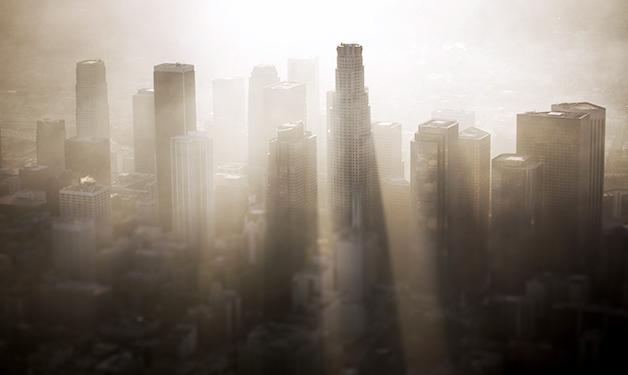
\includegraphics[height=6em]{logo_left}} 
  % Title
  {{\bf\textsc{Air pollutioution - the problem for generation}\vspace{0.5em}} \\ \scalebox{.7}{The Effect of Ambient Air Particulate Matter to the Sperm Epigenome}}
  % Authors
  {\textsc{Team \#5}}
  % University logo
  {% The makebox allows the title to flow into the logo, this is a hack because of the L shaped logo.
    
\includegraphics[height=9.0em]{logo_wsci}
  }

%%%%%%%%%%%%%%%%%%%%%%%%%%%%%%%%%%%%%%%%%%%%%%%%%%%%%%%%%%%%%%%%%%%%%%%%%%%%%%
%%% Now define the boxes that make up the poster
%%%---------------------------------------------------------------------------
%%% Each box has a name and can be placed absolutely or relatively.
%%% The only inconvenience is that you can only specify a relative position 
%%% towards an already declared box. So if you have a box attached to the 
%%% bottom, one to the top and a third one which should be in between, you 
%%% have to specify the top and bottom boxes before you specify the middle 
%%% box.
%%%%%%%%%%%%%%%%%%%%%%%%%%%%%%%%%%%%%%%%%%%%%%%%%%%%%%%%%%%%%%%%%%%%%%%%%%%%%%
    %
    % A coloured circle useful as a bullet with an adjustably strong filling
    \newcommand{\colouredcircle}{%
      \tikz{\useasboundingbox (-0.2em,-0.32em) rectangle(0.2em,0.32em); \draw[draw=black,fill=lightblue,line width=0.03em] (0,0) circle(0.18em);}}

%%%%%%%%%%%%%%%%%%%%%%%%%%%%%%%%%%%%%%%%%%%%%%%%%%%%%%%%%%%%%%%%%%%%%%%%%%%%%%
  \headerbox{Introduction}{name=introduction,column=0,row=0}{
%%%%%%%%%%%%%%%%%%%%%%%%%%%%%%%%%%%%%%%%%%%%%%%%%%%%%%%%%%%%%%%%%%%%%%%%%%%%%%
You know that air pollution is affecting millions of people around the world, but how exactly?


Your brain, your heart, and most of all your lungs suffer every day, but there is something so small yet so important, that affects you and the generations you will give life to. So far researches have focused on {\bf macroscopic level} (vital organs, blood etc.) but now something new and far more concerning has surfaced. The newest discoveries of the scientific world show that certain particles in the air due to pollution can damage our genetic system.  These particles don't change the {\bf DNA} sequence directly but influence the process of genetic expression explained by a growing field of molecular biology, epigenetics. {\bf Epigenetics} is the study of changes in variation in the genetic material specifically gene expression that is attributed to external environmental factors. This phenomena does not only produce a present and concerning problem, but also a future one. This field is specifically called {\bf trans-generational epigenetics} which could be both maternal and paternal. Exposure to air pollution has long been connected to male infertility and low sperm quality but a deeper molecular understanding of the mechanism on how it occurs is poorly understood. Studies conducted on sperm have showed that the epigenetic changes in sperm cells is passed on to offspring after successful fertilization, thus this problem perpetuates on the next generations.
   \vspace{0.3em}
 }

%%%%%%%%%%%%%%%%%%%%%%%%%%%%%%%%%%%%%%%%%%%%%%%%%%%%%%%%%%%%%%%%%%%%%%%%%%%%%%
  \headerbox{Aims/Objectives}{name=contribution,column=0,row=0,below=introduction,above=bottom}{
%%%%%%%%%%%%%%%%%%%%%%%%%%%%%%%%%%%%%%%%%%%%%%%%%%%%%%%%%%%%%%%%%%%%%%%%%%%%%%
  The study generally aims to find a correlation between a person's exposure to air pollution and the stability of his or her genetic information. Furthermore, to look at the possibility of affecting the next generation. Specifically, the study will look into the effect of exposure to air pollution to the number of {\bf epigenetic markers} change for a specific observation time.
   \vspace{0.3em}
  }

%%%%%%%%%%%%%%%%%%%%%%%%%%%%%%%%%%%%%%%%%%%%%%%%%%%%%%%%%%%%%%%%%%%%%%%%%%%%%%
  \headerbox{References}{name=references,column=3,above=bottom}{
%%%%%%%%%%%%%%%%%%%%%%%%%%%%%%%%%%%%%%%%%%%%%%%%%%%%%%%%%%%%%%%%%%%%%%%%%%%%%%
    \smaller
    \bibliographystyle{ieee}
    \renewcommand{\section}[2]{\vskip 0.05em}
    \nocite{*}
    \bibliography{biblio}
    %   \begin{thebibliography}{1}\itemsep=-0.01em
    %   \setlength{\baselineskip}{0.4em}
    %   \bibitem{amberg11:graphtrack}
    %     B.~Amberg, T. Vetter.
    %     \newblock {GraphTrack}: {F}ast and {G}lobally {O}ptimal {T}racking in {V}ideos
    %     \newblock In {\em CVPR '11}
    %   \bibitem{awf:tracking}
    %     A.~Buchanan and A.~Fitzgibbon.
    %     \newblock {I}nteractive {F}eature {T}racking using {K-D} {T}rees and {D}ynamic {P}rogramming.
    %     \newblock In {\em CVPR '06}
    %   \end{thebibliography}
    
   \vspace{0.3em}
  }

%%%%%%%%%%%%%%%%%%%%%%%%%%%%%%%%%%%%%%%%%%%%%%%%%%%%%%%%%%%%%%%%%%%%%%%%%%%%%%
\headerbox{ \scalebox{.9}{Conclusions and Implications}}{name=speed,column=3,span=1}{
  %%%%%%%%%%%%%%%%%%%%%%%%%%%%%%%%%%%%%%%%%%%%%%%%%%%%%%%%%%%%%%%%%%%%%%%%%%%%%%
  \noindent 
  \textbullet~The data could suggest the effect of exposure to certain concentrations of ambient air particulate matter to the number of epigenetic marker changed for an observation time. Furthermore, any epigenetic changes observed could indicate the possibility of affecting offspring on concerned individuals on whatever mechanism of gene expression the epigenetic marker is responsible for.\\
  \textbullet~The study could also provide a way of better understanding the sperm epigenome and how it is externally affected. Also, this could lead to possible mechanisms of explaining infertility problems, neonatal deaths, fetal development and paternal contributions to offspring.
  \vspace{0.2em}
  }
%%%%%%%%%%%%%%%%%%%%%%%%%%%%%%%%%%%%%%%%%%%%%%%%%%%%%%%%%%%%%%%%%%%%%%%%%%%%%%
  \headerbox{Method}{name=method,column=1,row=0,span=2}{
%%%%%%%%%%%%%%%%%%%%%%%%%%%%%%%%%%%%%%%%%%%%%%%%%%%%%%%%%%%%%%%%%%%%%%%%%%%%%%
  \noindent
  \begin{tabular}{  p{1.6cm} p{13.cm} }
   {\bf Study \newline population} & \textbullet~A city with a {\bf monitoring system} for ambient air particulate matter would be chosen.\\    
   & \textbullet~{\bf 200 men} of reproductive age, {\bf 18 to 40 years}, would be selected at random.\\
   & \textbullet~Each person will be enrolled in a {\bf regular check-up program} for the monitoring current health status and lifestyle.\\
   & \textbullet~For each check-up, a participant will also answer a comprehensive {\bf questionnaire} which includes inquiries on information regarding the patient's condition.\\
   & \textbullet~Semen samples, for {\bf sperm epigenome analysis}, will also be collected from each participant.\\

    \hline
    {\bf Exposure {\it PM}} & \textbullet~Data on exposure to ambient air particulate matter will be based on amount of time a person stays in the area (gathered through questionnaire) and the concentration of particulate matter exposed to (gathered through monitory system machine). \\
    \arrayrulecolor{blue}\hline

    {\bf Health Status} & \textbullet~The patient's health status will be evaluated through regular check-up with a physician and lifestyle will be evaluated using a questionnaire.\\
    {\bf and Lifestyle} & \textbullet~This data will be used to eliminate biases related to the fact that epigenetic changes might be attributed to aging, lifestyle, etc. \\
    \arrayrulecolor{blue}\hline

    {\bf Epigenetic Changes in the Sperm}
    & \textbullet~The sperm cells from collected semen samples would be analyzed for specific epigenetic changes, following protocols of epigenetic analysis for the sperm epigenome. Epigenetic markers like {\bf DNA methylation} changes and other {\bf post-transcriptional modifications} like histones among others would be considered.\\
    & \textbullet~Epigenetic changes will be quantified as the number of epigenetic marker changed for an observation event.\\
    \arrayrulecolor{blue}\hline

    {\bf Data \newline Integration} & \textbullet~For every participant, 3 general data point should be gathered for each data collection event: exposure, current health status and epigenetic changes in the sperm.

  \end{tabular}
   % \vspace{0.3em}
  }

\headerbox{Deaths attributable to outdoor air pollution, 2008}{name=dead_map,column=1,row=0,span=2,below=method}{
  \noindent{\centering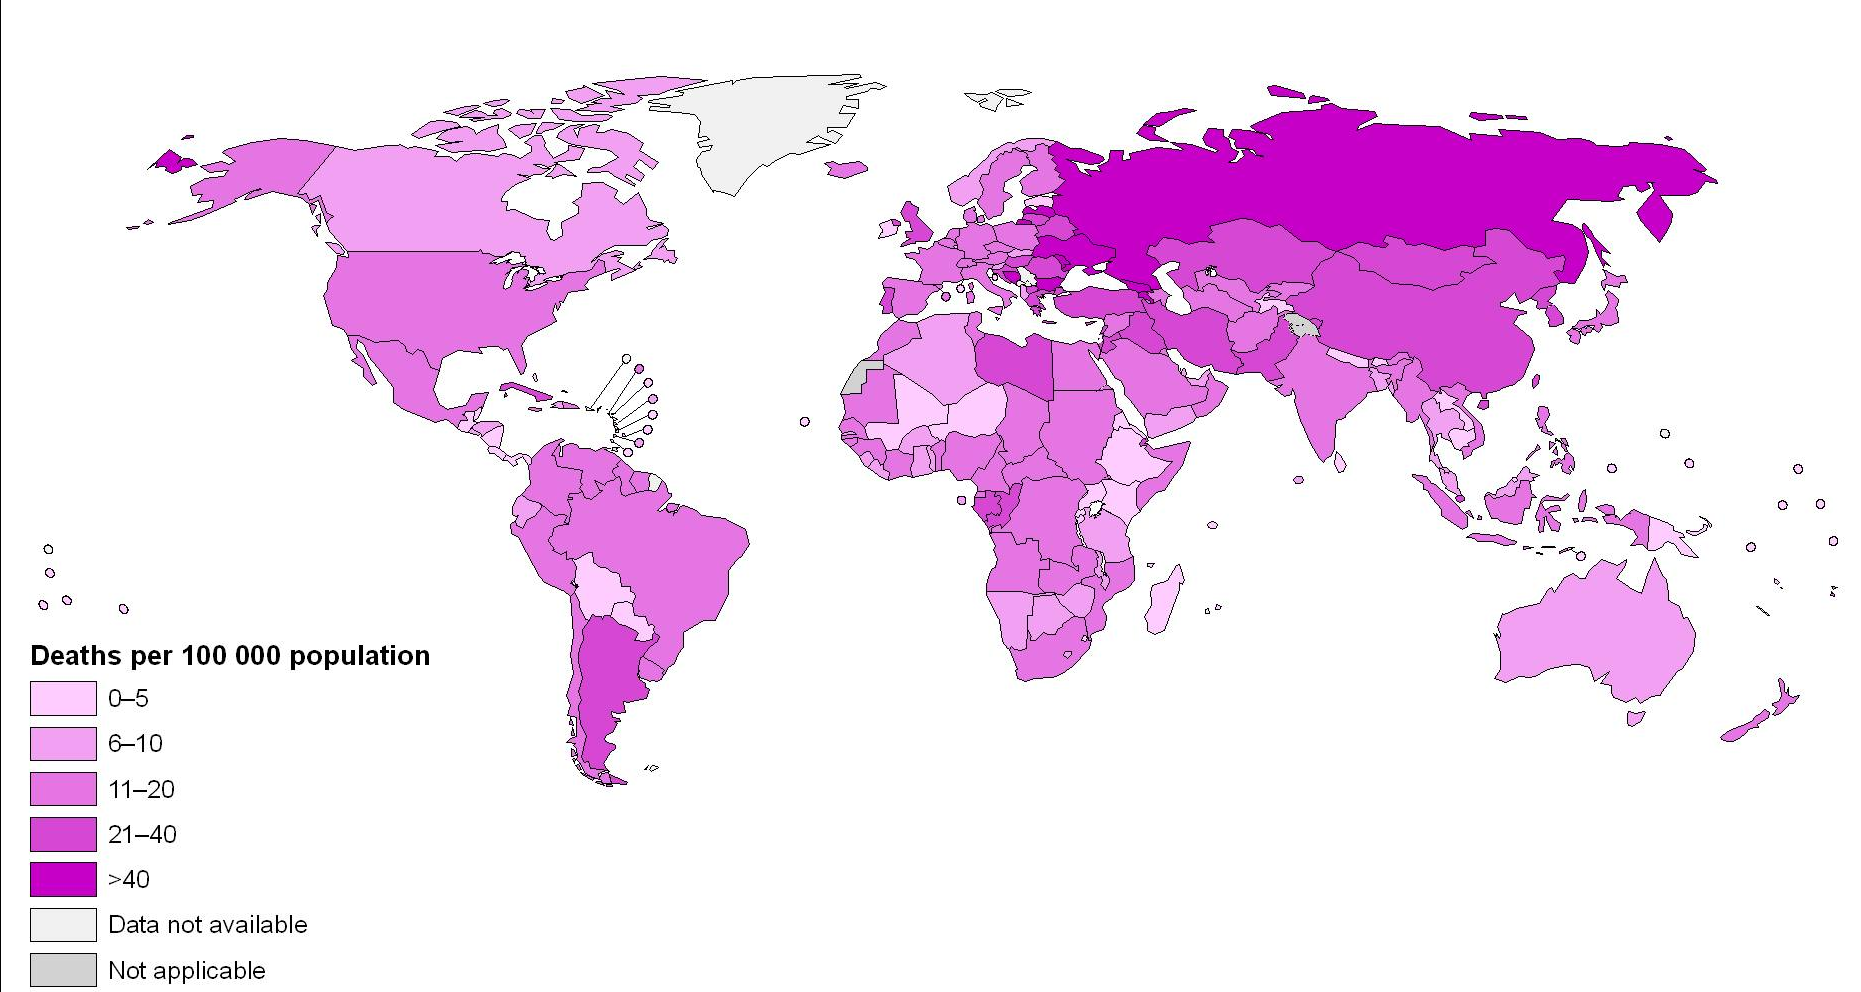
\includegraphics[width=0.95\linewidth]{air_pollution_map_min}}
}

%%%%%%%%%%%%%%%%%%%%%%%%%%%%%%%%%%%%%%%%%%%%%%%%%%%%%%%%%%%%%%%%%%%%%%%%%%%%%%
\headerbox{Future works}{name=future_works,column=3,span=1,row=0,below=speed,above=references}{
  If the affection of air pollution to DNA is real, then Machine Learning techniques could be used on the data obtained for classifier creation. In the same time Data Mining techniques  could give smart statistical analysis of the data and find scalable correlations of air pollution and epigenetic disease for specific city. \\
  \indent {\bf Output}:\\
  \indent \textbullet~The classifier could predict if in currently a city has influential air pollution to DNA of the citizens in general: YES, NO (the simplest version of classifier);\\
  \indent \textbullet~more complex prediction model that is based on non-linear relation(like neural nets) could give measurable output for some Epigenetic interests.\\
  \indent{\bf Input Data from}:\\
    \indent \textbullet~random 150 male citizens with reproductive age 18-40 years old;\\
    \indent \textbullet~while one year with period every 2 month.
  
}

\end{poster}

\end{document}